\section{Methodology} \label{sec:methodology}


\subsection{Lab Objectives and Workflow}

The primary goal of this lab is to develop a machine 
learning approach for estimating the masses of galaxy 
clusters directly from X-ray image data. We begin with a 
simple regression task, using a convolutional neural network
(CNN) to predict the cluster mass from the simulated images. 
As we progressed, we encountered challenges such as overfitting 
and limited generalization, this motivated us to use various 
regularization techniques—including dropout, batch normalization,
and data augmentation—which we discuss in subsequent sections.

After improving the basic model with regularization, we 
incorporated additional astrophysical features, such as the 
cluster redshift, to further enhance the predictive performance. 
We systematically evaluated each model by training on a split 
dataset (training, validation, and test sets) and assessed the
results through scatter plots of predicted versus true masses. 
Finally, we extended the network to predict not only the mean 
mass but also its uncertainty, by modeling the output as a 
Gaussian distribution and training with a log-likelihood loss. 




\subsection{Data Preparation and Preprocessing}

\paragraph{Data loading.}


The dataset used in this lab consists of simulated galaxy 
clusters based on the eROSITA Final Equatorial-Depth Survey (eFEDS \cite{eFEDS_V3}). 
Specifically, 
the X-ray images and associated catalogues are derived from mock
event files and simulations that mimic the expected performance 
and observational properties of eROSITA prior to its all-sky survey. 
These simulations were designed to reproduce realistic data,
and have been processed with detection and extent 
likelihood cuts to select a high-quality sample of clusters.

Each cluster is represented by a simulated X-ray image of shape 
$50\times50\times10$, where $50\times50$ are the pixel dimensions and
$10$ is the number of energy channels (bands) per image. 
The dataset contains a total of 7,946 such cluster images:
\begin{itemize}
    \item Number of clusters: $N = 7,946$
    \item Image shape: $50 \times 50 \times 10:$(height $\times$ width $\times$ energy bands)
\end{itemize}

For each cluster, these are the available featuers extracted from the dataset:

\begin{itemize}
    \item \textbf{index} -- Unique integer index of the cluster
    \item \textbf{SRC\_ID\_IN} -- Source identification number (input)
    \item \textbf{RA}, \textbf{DEC} -- Right Ascension and Declination (sky coordinates)
    \item \textbf{z} -- Redshift
    \item $kT$ -- Plasma temperature (keV)
    \item $d_L$ -- Luminosity distance
    \item $L_{X,\mathrm{soft}}$, $L_{X,\mathrm{soft}}^{2R_{500}}$ -- X-ray luminosity in the soft band (total and within $2R_{500}$)
    \item $F_{X,\mathrm{soft}}$, $F_{X,\mathrm{soft}}^{2R_{500}}$ -- X-ray flux in the soft band (total and within $2R_{500}$)
    \item $M_{500c}$ -- Cluster mass within $R_{500c}$
    \item $R_{500c}^{\mathrm{arcmin}}$, $R_{500c}^{\mathrm{kpc}}$ -- Cluster radius $R_{500c}$ in arcminutes and kiloparsecs
    \item \textbf{pid} -- Process ID
    \item $M_{\mathrm{vir}}$, $R_{\mathrm{vir}}$ -- Virial mass and virial radius
    \item $X_{\mathrm{off}}$ -- Offset of cluster center
    \item $b/a_{500c}$ -- Minor-to-major axis ratio within $R_{500c}$
    \item \textbf{ID\_SRC\_OUT} -- Source ID (output)
    \item $\mathrm{RA}_{\mathrm{eSASS}}$, $\mathrm{DEC}_{\mathrm{eSASS}}$ -- Coordinates from eSASS pipeline
    \item $\mathrm{RADEC}_{\mathrm{ERR}}$ -- Uncertainty in sky position
    \item \textbf{EXT}, \textbf{EXT\_ERR}, \textbf{EXT\_LIKE} -- Source extent, uncertainty, and likelihood
    \item $\mathrm{ML}_{\mathrm{RATE}}$, $\mathrm{ML}_{\mathrm{RATE,ERR}}$ -- Maximum likelihood count rate and its error
    \item $\mathrm{DET}_{\mathrm{LIKE}}$ -- Detection likelihood
    \item $\mathrm{ML}_{\mathrm{BKG}}$, $\mathrm{ML}_{\mathrm{EXP}}$ -- Maximum likelihood background and exposure
    \item \textbf{input\_SRC\_ID} -- Input source identification number
    \item \textbf{Nreal} -- Number of real sources associated
    \item $\mathrm{CLU}_X$, $\mathrm{CLU}_Y$ -- Cluster X and Y pixel coordinates
\end{itemize}

These features include the cluster's properties 
(such as mass, redshift, X-ray luminosity), sky position (RA, DEC) and
error measurements

\begin{figure}[H]
    \centering
    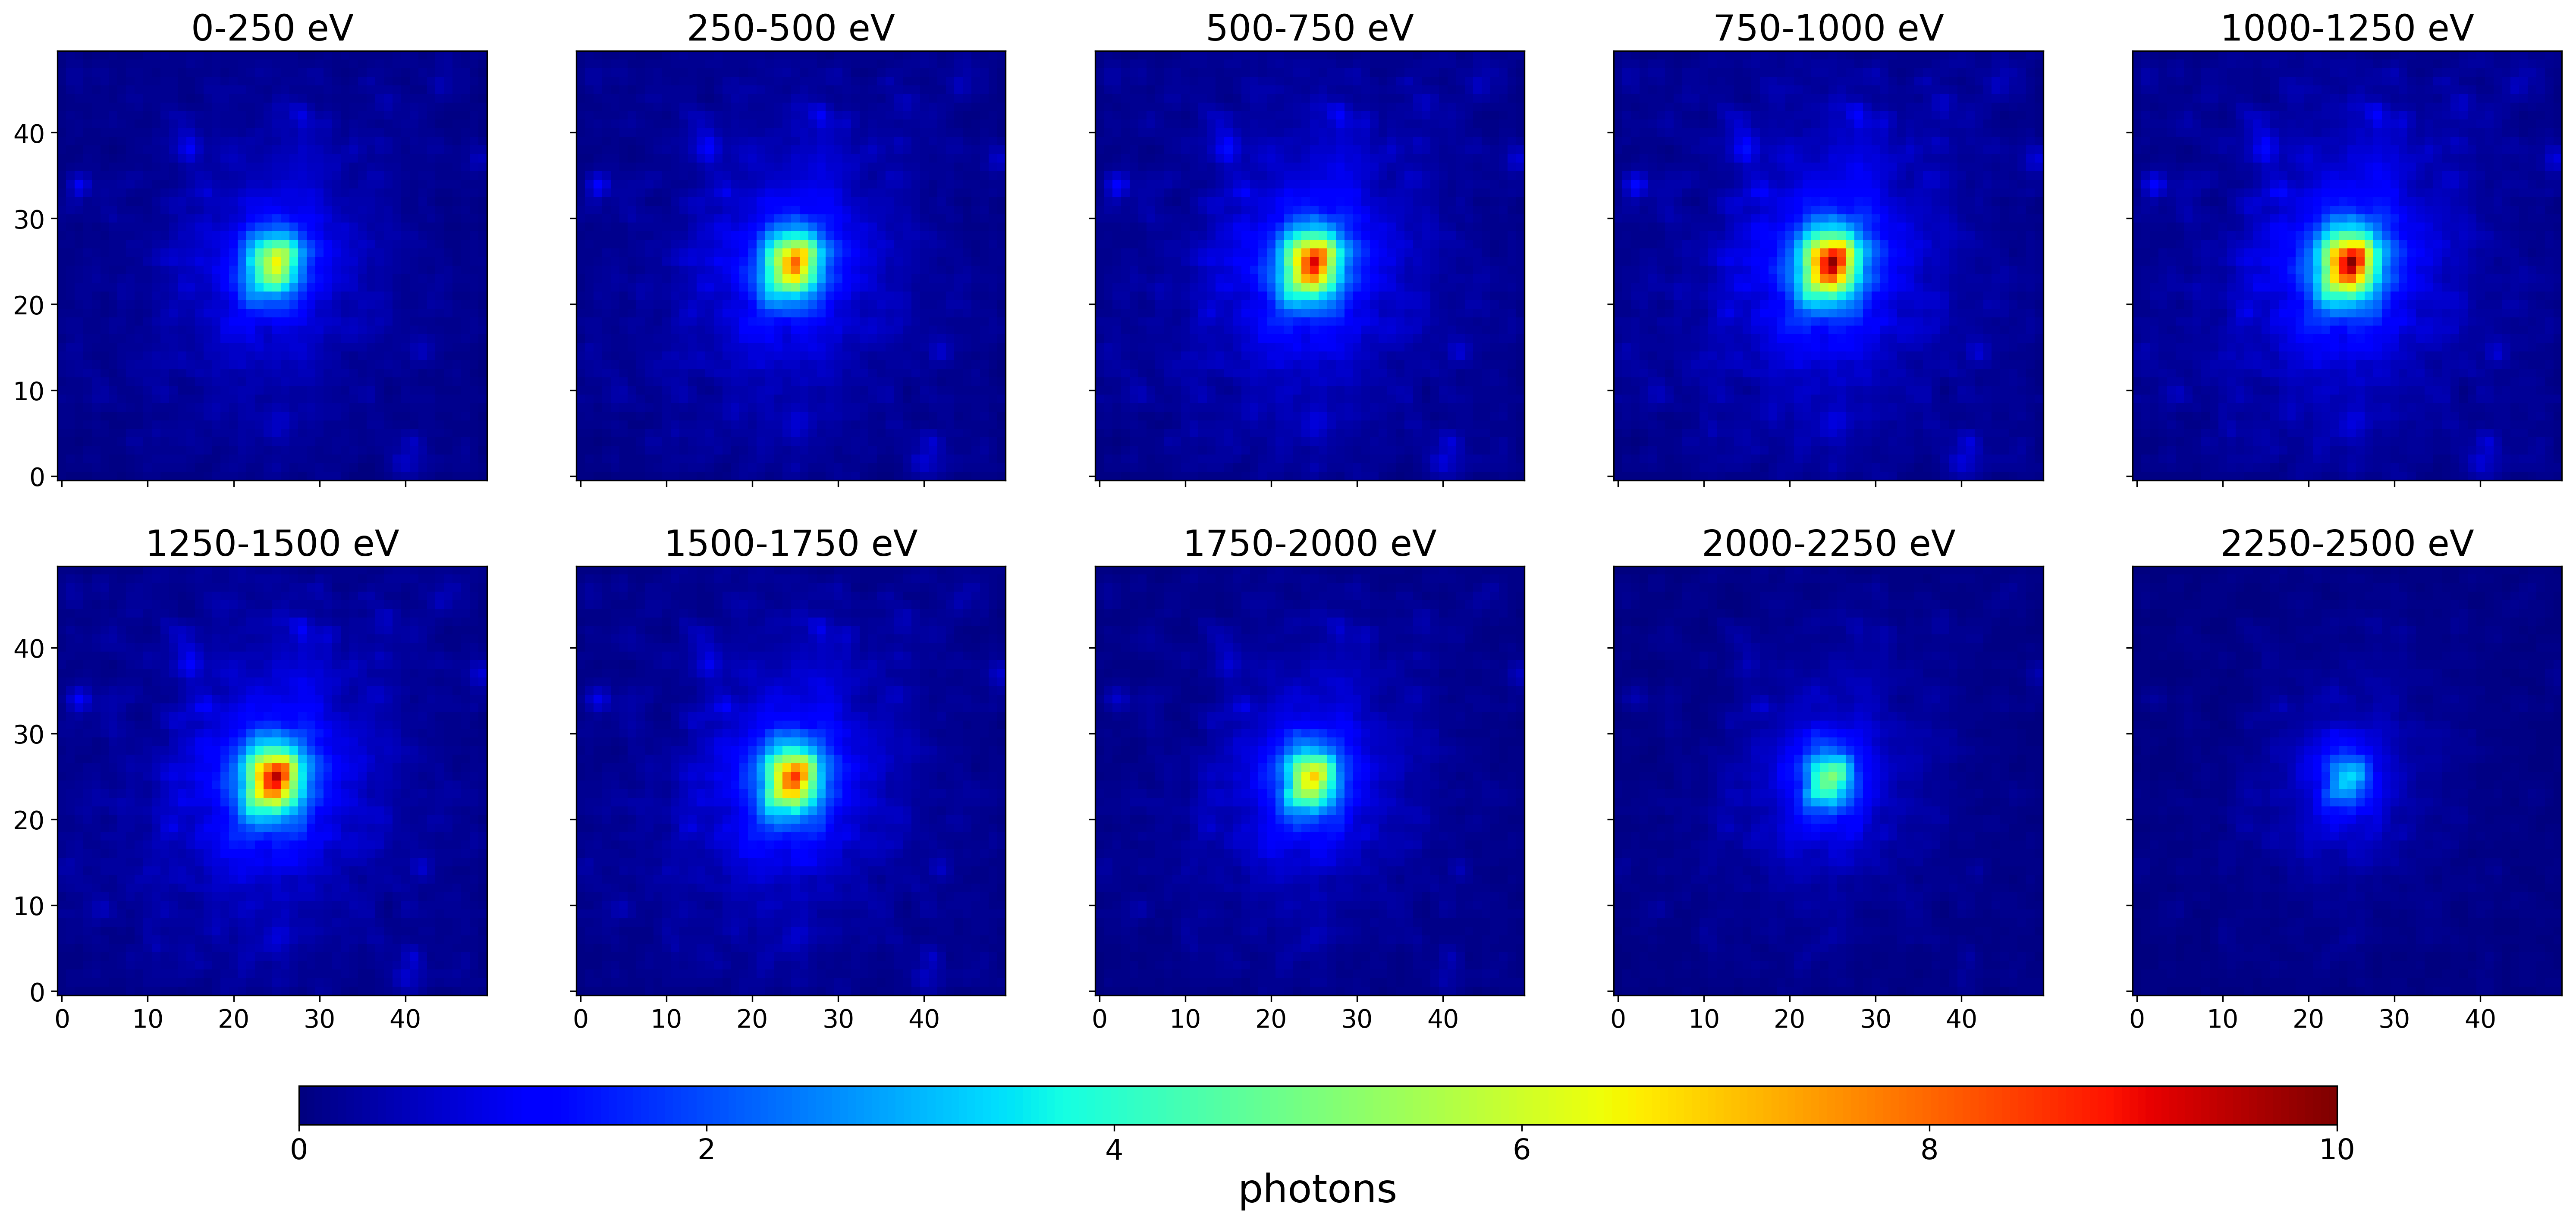
\includegraphics[width=0.7\linewidth]{chapters/methodology/efeds_energy_image.png}
    \caption{Example of a simulated X-ray image from the eFEDS 
    dataset used in this lab. The image represents 
    the photon energy distribution for a mock galaxy cluster, for several different,
    energy bands.}
    \label{fig:efeds_example}
\end{figure}

Data loading is handled by a dedicated \texttt{data laoder} class, 
which parses the image and catalog files and returns a NumPy
array of images  and a dictionary of features for each cluster.


\paragraph{Feature normalization.}
Before training, each feature used
(such as cluster mass and redshift) is  normalized to have zero 
mean and unit variance:

\[
x_{\text{norm}} = \frac{x - \mu}{\sigma}
\]

where $\mu$ and $\sigma$ are the mean and standard deviation computed 
from the training data. This normalization ensures numerical 
stability -- large outliers are normlaized and do not have big impact
either on the training nor the evaluation of our model.
The normalization parameters 
are stored, enabling inverse transformation (“denormalization”)
for interpretation of model predictions.
The denormalization was necessary in order to gain interpretable results of the mass,
since after normalizing all our results gather around zeron -- which makes 
no physical sense (zero mass?)

\paragraph{Image normalization.}
To account for variation in overall image intensity, 
each image is also normalized to zero mean and unit variance,
either per-image or per-channel. In this project, 
per-image normalization is used:
\[
I_{\text{norm}} = \frac{I - \langle I \rangle}{\sigma_I}
\]
where $\langle I \rangle$ and $\sigma_I$ are computed over all 
pixels and channels of the image.

\paragraph{Dataset splitting.}
The dataset is randomly partitioned into training, validation, and test sets using stratified splits:
\begin{itemize}
    \item 70\% for training
    \item 15\% for validation
    \item 15\% for testing
\end{itemize}
Splitting is performed using fixed random seeds for 
reproducibility.

\paragraph{Image augmentation.}
To improve generalization of our model we increase the
size of the training data, via performing image augmentation to the 
training images. Augmentation operations include random horizontal 
and vertical flips, small random rotations, random zoom, and random 
cropping. Further details of Image augmentation will be discussed in the 
models section \ref{sec:models}

\subsection{Negative Log-Likelihood Loss}

To enable the neural network to not only predict the cluster mass 
but also to estimate its uncertainty, we adopt a probabilistic 
approach. We model the predicted mass for each cluster as a 
Gaussian random variable with mean $\mu = f(x, \theta)$ and variance 
$\sigma^2 = \sigma(x, \theta)^2$ output by the neural network.

The likelihood for a single true mass value $y$ given input $x$ 
and network parameters $\theta$ is

\begin{equation}
    p(y|x, \theta) = \frac{1}{\sqrt{2\pi \sigma(x, \theta)^2}} \exp\left( -\frac{(y - f(x, \theta))^2}{2\sigma(x, \theta)^2} \right).
\end{equation}

During training, we wish to maximize the likelihood --
equivalently, \textbf{minimize} the negative log-likelihood
over the training set. The negative log-likelihood (NLL) 
for a single data point is:
\begin{equation}
    \mathcal{L}_{\mathrm{NLL}} = -\log p(y|x, \theta) = \frac{1}{2} \log \left(2\pi \sigma(x, \theta)^2\right) + \frac{(y - f(x, \theta))^2}{2\sigma(x, \theta)^2}
\end{equation}

In our implementation, the neural network is designed so 
that the output for each sample consists of two values: 
the predicted mean $\mu$ (for the mass) and the predicted 
variance $\sigma^2$ (for the uncertainty). The loss function 
used in training is the average NLL over all samples in a batch:
\begin{equation}
    \mathrm{loss}_{\mathrm{NLL}} = \frac{1}{N} \sum_{i=1}^N \left[ \frac{1}{2} \log \left(\sigma_i^2 + \epsilon\right) + \frac{(y_i - \mu_i)^2}{2 (\sigma_i^2 + \epsilon)} \right]
\end{equation}
where $\epsilon$ is a small constant ("jitter") added for numerical 
stability (no divisions by 0). An attentive reader could observe that there is 
a term missing, however the "$\pi$" term is ommitted as it is just a constant!
The code implementation of the NLL can be seen in the Appendix \ref{appendix:nll}

\subsection{Coverage: Evaluating Predictive Uncertainty}
\label{sec:coverage}

When our neural network predicts both a mean value and an associated 
standard deviation for the target variable (e.g., cluster mass), 
it is important to assess whether these predicted uncertainties 
are calibrated---that is, whether they accurately reflect the true 
variability in the data.

The metric we use is coverage,
which quantifies the fraction of true target values that 
fall within a predicted confidence interval. We use a 
symmetric interval defined by the predicted mean $\mu$ and 
predicted standard deviation 
$\sigma$ (i.e., $[\mu - \sigma,\, \mu + \sigma]$), the  coverage 
is given by:

\begin{equation}
\mathrm{Coverage} = \frac{1}{N} \sum_{i=1}^N \mathbb{I} \left( y_i^\mathrm{true} \in [\mu_i - \sigma_i,\, \mu_i + \sigma_i] \right),
\end{equation}
where $\mathbb{I}$ is the indicator function, $N$ is the number of 
test examples, $y_i^\mathrm{true}$ is the true target value, 
and $(\mu_i, \sigma_i)$ are the predicted mean and standard deviation 
for the $i$-th sample.


\subsection{Pull Distribution}
\label{subsec:pull}

We use another helpfull metric, in order to assess not 
only the accuracy but also the calibration of our predicted 
uncertainties, we analyze the distribution of the \textit{pull} values. 
The pull for each test sample is defined as
\begin{equation}
\mathrm{Pull} = \frac{y_\mathrm{true} - \mu_\mathrm{pred}}{\sigma_\mathrm{pred}},
\end{equation}

where $y_\mathrm{true}$ is the true target value, 
$\mu_\mathrm{pred}$ is the predicted mean, 
and $\sigma_\mathrm{pred}$ is the predicted standard 
deviation (uncertainty) for each test point.

Ideally, if the model is both accurate and well-calibrated, 
the distribution of pull values across the test set should be 
centered around zero (then we have unbiased predictions) and have a standard 
deviation close to one.


\subsection{Regularization and Normalization Techniques}

To achieve better generalization and stable training, 
our most successful convolutional neural network models 
employ several normalization and regularization techniques:

\begin{itemize}
    \item \textbf{Batch Normalization}: Batch normalization layers are applied after convolutional 
    and dense layers to normalize intermediate activations. 
    This accelerates and achieves a more stable and faster convergence
    \item \textbf{Dropout}: Dropout is used in the fully connected (dense) layers to prevent overfitting 
    by randomly deactivating a subset of neurons during training.
    \item \textbf{Max Pooling}: Max pooling layers are inserted between convolutional layers to 
    downsample feature maps, reducing the spatial dimensions and encouraging the network to learn 
    translation-invariant features. 
    \item \textbf{Padding}: ``Same'' padding is used in convolutional layers to maintain the spatial 
    resolution of the input throughout the network.
\end{itemize}

The aforementioned techniques help prevent overfitting, 
promote generalization, and ensure that our models can extract meaningful
patterns from the data without memorizing noise. 

\subsection{Hyperparameter Optimization with Optuna}

To identify the optimal architecture and training configuration for our 
convolutional neural network, we performed a hyperparameter 
search using the \texttt{Optuna} framework. 

In each Optuna trial, a new model configuration is sampled from a 
predefined search space, trained on the training set, and evaluated on 
the validation set. The objective metric minimized during optimization was 
the mean squared error (MSE) on the validation set.

In our study, we employed two different loss functions at 
different stages of model development. During hyperparameter 
optimization with Optuna, we minimized the mean squared error 
(MSE) on the validation set (while having the NLLloss). MSE is a 
was chosen for this regression 
task, as it is easy to interpret and provides a direct measure of 
prediction accuracy for the target variable. 

Thus, while MSE was used for hyperparameter search due to its 
simplicity and interpretability, the final models were trained 
and evaluated with the NLL loss to make full use of the model's 
capabilities.


The following hyperparameters were tuned in our study:

\begin{itemize}
    \item \textbf{Input Features:} We tested combinations of additional scalar features appended to the image input, including redshift (\texttt{z}), temperature (\texttt{kT}), and soft-band X-ray luminosity (\texttt{Lx\_soft}).
    \item \textbf{Convolutional Layers:} The number of convolutional layers (2--4), number of filters per layer (16, 32, 64, 128), kernel sizes (\{10$\times$10, 5$\times$5, 3$\times$3, 2$\times$2\}), use of max pooling, and application of batch normalization were all varied independently.
    \item \textbf{Fully Connected Layers:} The number of dense (fully connected) layers (1--2), units per layer (64, 128, 256), inclusion of batch normalization and dropout, and dropout rates (0.2--0.5) were explored.
    \item \textbf{Head Layers:} The number of head layers (1--2), units per layer (64, 128, 256), use of batch normalization and dropout, and dropout rates (0.2--0.5).
    \item \textbf{Learning Rate:} The learning rate for the Adam optimizer was tuned on a logarithmic scale in the range $[10^{-4}, 10^{-2}]$.
    \item \textbf{Data Augmentation:} We tested whether to apply random image augmentations during training or not.
\end{itemize}

At each trial, the model was trained for up to 100 epochs with early 
stopping --with patience 20 and evaluated on the validation set. Results from all trials were periodically checkpointed and saved for reproducibility and further analysis.


\subsection{Training Procedure}

For training the final models, we used the Adam optimizer, 
the models were trained to minimize the negative log-likelihood (NLL) loss function 
in order to predict 
both the mean and uncertainty (variance) of the target mass 
for each galaxy cluster. As a metric for monitoring model 
performance during training, we tracked the mean squared error 
(MSE) on the training and validation sets.

We trained all models using a batch size of 64, for up to 100 
epochs, and employed early stopping with a patience of 20 epochs. 

